\documentclass{beamer}

% Font selection
\usepackage{palatino}

% Beamer template
\usetheme{Antibes}
%\usetheme{Berlin}

\usepackage[scale=1.2]{ccicons}

\usepackage[utf8]{inputenc}
\usepackage[T1]{fontenc}
\usepackage[spanish]{babel}

\usepackage{tabularx}
\usepackage{multicol}
\usepackage{minted}
\usepackage{graphicx}

\usepackage{listings}

\lstset{
  language=C++,
  columns=flexible,
  identifierstyle=\itshape,
%
  belowcaptionskip=1\baselineskip,
  breaklines=true,
  xleftmargin=\parindent,
  language=C++,
  showstringspaces=false,
  basicstyle=\tiny,
  keywordstyle=\bfseries\color{green!40!black},
  commentstyle=\itshape\color{purple!40!black},
  identifierstyle=\color{blue},
  stringstyle=\color{brown},
  columns=flexible,
%  inputenconding=utf8,
  extendedchars=true,
%
  morekeywords=[1]{constexpr,nullptr,alignof,alignas,decltype},
  literate={%
    {¿}{{?`}}1
    {¡}{{!`}}1
    {á}{{\'a}}1
    {é}{{\'e}}1
    {í}{{\'i}}1
    {ó}{{\'o}}1
    {ú}{{\'u}}1
    {ñ}{{\~n}}1
}
}

\newcommand{\cppkey}[1]{%
{\color{green!40!black}\texttt{#1}}%
}

\newcommand{\cppid}[1]{%
{\color{blue}\texttt{#1}}%
}

\lstdefinestyle{terminal}{
  language=bash,
  basicstyle=\scriptsize\ttfamily,
  numbersep=3pt,
  frame=tb,
  columns=fullflexible,
  backgroundcolor=\color{yellow!20},
  literate=%
    {¿}{{?`}}1
    {¡}{{!`}}1
    {á}{{\'a}}1
    {é}{{\'e}}1
    {í}{{\'i}}1
    {ó}{{\'o}}1
    {ú}{{\'u}}1
    {ñ}{{\~n}}1
}


\usepackage{listings}

\lstdefinestyle{terminal}{
  language=bash,
  basicstyle=\scriptsize\ttfamily,
  numbersep=3pt,
  frame=tb,
  columns=fullflexible,
  backgroundcolor=\color{yellow!20},
  literate=%
    {¿}{{?`}}1
    {¡}{{!`}}1
    {á}{{\'a}}1
    {é}{{\'e}}1
    {í}{{\'i}}1
    {ó}{{\'o}}1
    {ú}{{\'u}}1
    {ñ}{{\~n}}1
}

\lstdefinestyle{termoutput}{
  basicstyle=\scriptsize\ttfamily,
  frame=tb,
  backgroundcolor=\color{blue!20},
  keywordstyle=\color{black},
  commentstyle=\color{black},
  identifierstyle=\color{black},
  stringstyle=\color{black},
}


\lstset{
  language=[ISO]C++,
  basicstyle=\scriptsize,
  morekeywords=[1]{constexpr,nullptr,alignof,alignas,decltype},
}


\renewcommand{\cppkey}[1]{%
{\color{green!40!black}\textbf{#1}}%
}

\renewcommand{\cppid}[1]{%
{\color{blue}\textbf{#1}}%
}


\usepackage{tikz}
\usetikzlibrary{positioning}
\usetikzlibrary{arrows}
\usetikzlibrary{mindmap}

\usepackage{pgfplots}
\pgfplotsset{compat=1.5}


\newcommand{\textgood}[1]{%
{\color{blue}\textbf{#1}}%
}

\newcommand{\textbad}[1]{%
{\color{red}\textbf{#1}}%
}

\newcommand{\textenum}[1]{%
{\color{blue!60!black}\textbf{#1}}%
}

\newcommand{\textmark}[1]{%
{\color{orange!70!black}\textbf{#1}}%
}




% Footline in every slide
\setbeamertemplate{footline}{
  \leavevmode%
  \hbox{\begin{beamercolorbox}[wd=\paperwidth,ht=2.5ex,dp=1.125ex,leftskip=.3cm,rightskip=.3cm]{author in head/foot}%
    \usebeamerfont{author in head/foot}\ccbyncndeu 
     \quad -- \quad J. Daniel Garcia 
     -- ARCOS@UC3M (\textbf{\url{josedaniel.garcia@uc3m.es}}) 
     -- Twitter: \textbf{\url{@jdgarciauc3m}}
    \hfill
    \insertframenumber/\inserttotalframenumber
  \end{beamercolorbox}}%
  \vskip0pt%
}

% Logo in every slide
\addtobeamertemplate{headline}{}
{% 
\begin{tikzpicture}[remember picture,overlay]
\node[anchor=north east] at (current page.north east) {
\includegraphics[height=0.7cm]{logos/arcos_t.png}};
\end{tikzpicture}
}

\tikzset{
  invisible/.style={opacity=0},
  visible on/.style={alt=#1{}{invisible}},
  alt/.code args={<#1>#2#3}{%
    \alt<#1>{\pgfkeysalso{#2}}{\pgfkeysalso{#3}} % \pgfkeysalso doesn't change the path
  },
}

%Portada
\title{Google Test + gcover}
\subtitle{Testing and measuring coverage in C++}
\author{J. Daniel Garcia}
\institute{ARCOS Group\\Universidad Carlos III de Madrid}
\date{}

\begin{document}

\begin{frame}
\titlepage
\end{frame}

\AtBeginSection[]
{
  \begin{frame}<*>
    \setbeamertemplate{section in toc shaded}[default][50]
    \setbeamertemplate{subsection in toc shaded}[default][50]
    \tableofcontents[currentsection,hideallsubsections]
  \end{frame}
}

\AtBeginSubsection[]
{
  \begin{frame}<beamer>
    \setbeamertemplate{subsection in toc shaded}[default][50]
    \tableofcontents[sectionstyle=show/hide,subsectionstyle=show/shaded/hide]
  \end{frame}
}

%\input{../config/license-cc.tex}
%\input{../config/arcos}
\section{Basic testing}

\subsection{Introduction}

\begin{frame}[t]{Examples}
\begin{itemize}
  \item You can get all the examples at:
\end{itemize}
\vspace{1cm}
\large
\textbf{\url{https://github.com/jdgarciauc3m/gtesttalk}}
\end{frame}

\begin{frame}[t]{What is Google Test?}
\begin{itemize}
  \item A library to perform unit testing in C++.
  
  \vfill
  \item \textenum{Features}:
    \begin{itemize}
      \item A \textmark{xUnit}-like framework.
      \item Test discovery.
      \item Variety on assertions.
      \item User defined assertions.
      \item \emph{Death tests}.
      \item Fatal and non-fatal failures.
      \item Value parametrized tests.
      \item Type parametrized tests.
      \item Multiple execution options.
      \item XML reporting.
    \end{itemize}

\end{itemize}
\end{frame}

\begin{frame}[t]{Use}
\begin{itemize}
  \item \textenum{Platforms}:
    \begin{itemize}
      \item Linux
      \item Mac OS X
      \item Windows
      \item Cygwin
      \item MinGW
      \item Windows Mobile
      \item Symbian
    \end{itemize}
  \vfill
  \item Some projects \textenum{using} it:
    \begin{itemize}
      \item \textmark{Chromium} Project.
      \item \textmark{LLVM} compiler family.
      \item \textmark{Protocol Buffers}.
      \item \textmark{OpenCV}.
    \end{itemize}
\end{itemize}
\end{frame}

\begin{frame}[t]{Principles}
\begin{enumerate}
  \item Tests should be \textmark{independent} and \textmark{repeatible}.
  \item Tests should be \textmark{well structured}.
  \item Tests should be \textmark{portable} y \textmark{reusable}.
  \item On failure, tests should give \textmark{maximum information}.
  \item Tests should not require writing \textmark{boilerplate code} for
        carrying out tests.
  \item Testing should be \textmark{fast}.
\end{enumerate}
\end{frame}

\begin{frame}[t,fragile]{How do I get Google Test?}
\begin{itemize}
  \item Repo in GitHub.
    \begin{itemize}
      \item \url{https://github.com/google/googletest}
    \end{itemize}
  \vfill
  \item You can get as a pakcage (Ubuntu/Linux).
    \begin{itemize}
      \item Package: \cppid{libgtest-dev}.
      \item \textbad{Important}: Does not intall binaries, only source code.
    \end{itemize}
\end{itemize}
\begin{lstlisting}[style=terminal]
$ apt-get install libgtest-dev
$ cd /usr/src/gtest
$ sudo mkdir build
$ cd build
$ sudo cmake ..
$ sudo make
$ sudo cp *.a /usr/lib
\end{lstlisting}
\end{frame}

\subsection{Example1: vectint}

\begin{frame}[t]{A vector of integers}
\begin{itemize}
  \item Let's start with a simple class.
  \item A vector of integers with minimal functionality:
    \begin{itemize}
      \item A vector of integers with a size (\cppid{size()}) 
            and maximum capacity (\cppid{capacity()}).
      \item Support for copy and move.
      \item Access \cppkey{operator[]}.
      \item Capacity modification (\cppid{reserve()}). 
      \item Size modification (\cppid{resize()}). 
    \end{itemize}
\end{itemize}
\end{frame}

\begin{frame}[t]{Interface}
\begin{block}{include/vectint.h}
\lstinputlisting[lastline=15]{examples/vector1/include/vectint.h}
\end{block}
\end{frame}

\begin{frame}[t]{Interface}
\begin{block}{include/vectint.h}
\lstinputlisting[firstline=16,lastline=26]{examples/vector1/include/vectint.h}
\end{block}
\end{frame}

\begin{frame}[t]{Interface}
\begin{block}{include/vectint.h}
\lstinputlisting[firstline=27]{examples/vector1/include/vectint.h}
\end{block}
\end{frame}

\begin{frame}[t]{Implementation}
\begin{block}{src/vectint.cpp}
\lstinputlisting[lastline=12]{examples/vector1/src/vectint.cpp}
\end{block}
\end{frame}

\begin{frame}[t]{Implementation}
\begin{block}{src/vectint.cpp}
\lstinputlisting[firstline=13,lastline=27]{examples/vector1/src/vectint.cpp}
\end{block}
\end{frame}

\begin{frame}[t]{Implementation}
\begin{block}{src/vectint.cpp}
\lstinputlisting[firstline=29,lastline=43]{examples/vector1/src/vectint.cpp}
\end{block}
\end{frame}

\begin{frame}[t]{Implementation}
\begin{block}{src/vectint.cpp}
\lstinputlisting[firstline=44]{examples/vector1/src/vectint.cpp}
\end{block}
\end{frame}

\begin{frame}[t]{Program using vectint}
\begin{columns}[T]

\column{.5\textwidth}
\begin{block}{samples/main1.cpp}
\lstinputlisting[lastline=13]{examples/vector1/samples/main1.cpp}
\end{block}

\column{.5\textwidth}
\begin{block}{samples/main1.cpp}
\lstinputlisting[firstline=14]{examples/vector1/samples/main1.cpp}
\end{block}

\end{columns}
\end{frame}




\subsection{Using CMake}

\begin{frame}[t]{What is CMake?}
\begin{itemize}
  \item A set of tools that allows to build, test and packages software.
  
    \begin{itemize}
      \item Starting from a CMake project you can generate scripts for
            building in each platform.
    \end{itemize}

  \item Generators:
    \begin{itemize}
      \item Makefiles (Unix, Borland, MinGW, NMake).
      \item Ninja.
      \item Visual Studio.
      \item Xcode.
      \item Several IDE:  CodeBlocks, CodeLite, EclipseCDT, KDevelop.
      \item IDE con soporte nativo: CLion, Visual.
    \end{itemize}
\end{itemize}
\end{frame}

\begin{frame}[t]{CMake root}
\begin{block}{CMakeLists.txt}\tiny
\inputminted{cmake}{examples/vector1/CMakeLists.txt}
\end{block}
\end{frame}

\begin{frame}[t]{CMake for src}
\begin{block}{src/CMakeLists.txt}\tiny
\inputminted{cmake}{examples/vector1/src/CMakeLists.txt}
\end{block}
\end{frame}

\begin{frame}[t]{CMake for samples}
\begin{block}{samples/CMakeLists.txt}\tiny
\inputminted{cmake}{examples/vector1/samples/CMakeLists.txt}
\end{block}
\end{frame}

\begin{frame}[t,fragile]{Building with CMake}
\begin{lstlisting}[style=terminal,basicstyle=\tiny\ttfamily]
jdgarcia@gavilan:~/vector1$ mkdir build
jdgarcia@gavilan:~/vector1$ cd build/
jdgarcia@gavilan:~/vector1/build$ cmake ..
-- The C compiler identification is GNU 6.2.0
-- The CXX compiler identification is GNU 6.2.0
-- Check for working C compiler: /usr/bin/cc
-- Check for working C compiler: /usr/bin/cc -- works
-- Detecting C compiler ABI info
-- Detecting C compiler ABI info - done
-- Check for working CXX compiler: /usr/bin/c++
-- Check for working CXX compiler: /usr/bin/c++ -- works
-- Detecting CXX compiler ABI info
-- Detecting CXX compiler ABI info - done
-- Configuring done
-- Generating done
-- Build files have been written to: /home/jdgarcia/vector1/build
\end{lstlisting}
\end{frame}

\begin{frame}[t,fragile]{What if I want to select the compiler?}
\begin{lstlisting}[style=terminal,basicstyle=\tiny\ttfamily]
jdgarcia@gavilan:~//vector1/build$ cmake .. -DCMAKE_CXX_COMPILER=clang++ -DCMAKE_C_COMPILER=clang
-- Configuring done
You have changed variables that require your cache to be deleted.
Configure will be re-run and you may have to reset some variables.
The following variables have changed:
CMAKE_C_COMPILER= clang
CMAKE_CXX_COMPILER= clang++

-- The C compiler identification is Clang 3.8.0
-- The CXX compiler identification is Clang 3.8.0
-- Check for working C compiler: /usr/bin/clang
-- Check for working C compiler: /usr/bin/clang -- works
-- Detecting C compiler ABI info
-- Detecting C compiler ABI info - done
-- Check for working CXX compiler: /usr/bin/clang++
-- Check for working CXX compiler: /usr/bin/clang++ -- works
-- Detecting CXX compiler ABI info
-- Detecting CXX compiler ABI info - done
-- Configuring done
-- Generating done
-- Build files have been written to: /home/jdgarcia//vector1/build
\end{lstlisting}
\end{frame}

\begin{frame}[t,fragile]{Compilation procedure}
\begin{lstlisting}[style=terminal,basicstyle=\tiny\ttfamily]
jdgarcia@gavilan:~/vector1/build$ make
Scanning dependencies of target dcl
[ 50%] Building CXX object src/CMakeFiles/dcl.dir/vectint.cpp.o
Linking CXX static library libdcl.a
[ 50%] Built target dcl
Scanning dependencies of target test1
[100%] Building CXX object samples/CMakeFiles/test1.dir/main1.cpp.o
Linking CXX executable ../test1
[100%] Built target test1
\end{lstlisting}
\end{frame}

\subsection{My first tests}

\begin{frame}[t]{Test cases and tests}
\begin{itemize}
  \item In Google Test we can define tests and group them in test cases.
    \begin{itemize}
      \item Use the macro \cppid{TEST}.
      \item \emph{Test case}: Elemental test.
      \item \emph{Test}: Each individual test forming the test case.
    \end{itemize}

  \vfill
  \item Performing checks:
    \begin{itemize}
      \item \cppid{EXPECT\_EQ}: Non fatal check.
      \item \cppid{ASSERT\_EQ}: Fatal check.
    \end{itemize}
\end{itemize}
\end{frame}

\begin{frame}[t]{Testing construction}
\begin{block}{utest/vectint\_constructor.cpp}
\lstinputlisting{examples/vector2/utest/vectint_constructor.cpp}
\end{block}
\end{frame}

\begin{frame}[t,fragile]{Running tests}
\begin{lstlisting}[style=terminal]
jdgarcia@gavilan:~/vector2/build$ ./vectint_utest 
Running main() from gtest_main.cc
[==========] Running 2 tests from 1 test case.
[----------] Global test environment set-up.
[----------] 2 tests from vectint_constructor
[ RUN      ] vectint_constructor.empty
[       OK ] vectint_constructor.empty (0 ms)
[ RUN      ] vectint_constructor.sized
[       OK ] vectint_constructor.sized (0 ms)
[----------] 2 tests from vectint_constructor (0 ms total)

[----------] Global test environment tear-down
[==========] 2 tests from 1 test case ran. (0 ms total)
[  PASSED  ] 2 tests.
\end{lstlisting}
\end{frame}

\begin{frame}[t,fragile]{Testing copy}
\begin{columns}[T]

\column{.5\textwidth}
\begin{block}{utest/vectint\_copy.cpp}
\lstinputlisting[lastline=15]{examples/vector2/utest/vectint_copy.cpp}
\end{block}

\column{.5\textwidth}
\begin{block}{utest/vectint\_copy.cpp}
\lstinputlisting[firstline=17]{examples/vector2/utest/vectint_copy.cpp}
\end{block}
\end{columns}
\end{frame}

\begin{frame}[t]{Configuring test compilation}
\begin{block}{utest/CMakeLists.txt}\tiny
\inputminted{cmake}{examples/vector2/utest/CMakeLists.txt}
\end{block}
\end{frame}

\begin{frame}[t,fragile]{Integrating tests in CMake}
\begin{itemize}
  \item It is enough to add an invocation to \cppid{enable\_testing()} 
        before including the tests directory.
\end{itemize}

\vfill
\begin{block}{CMakeLists.txt}\small
\begin{minted}{cmake}
#...
enable_testing()
add_subdirectory(utest)
\end{minted}
\end{block}

\vfill
\begin{itemize}
  \item A new target is generated for running tests.
    \begin{itemize}
      \item \cppkey{make test}.
      \item \cppkey{ctest}.
    \end{itemize}
\end{itemize}
\end{frame}

\begin{frame}[t,fragile]{Running the tests}
\begin{lstlisting}[style=terminal]
jdgarcia@gavilan:~/github-repos/examples/gtesttalk/vector2/build$ make test
Running tests...
Test project /home/jdgarcia/github-repos/examples/gtesttalk/vector2/build
    Start 1: vectint_copy.copy_construct
1/4 Test #1: vectint_copy.copy_construct ......   Passed    0.00 sec
    Start 2: vectint_copy.copy_assign
2/4 Test #2: vectint_copy.copy_assign .........   Passed    0.00 sec
    Start 3: vectint_constructor.empty
3/4 Test #3: vectint_constructor.empty ........   Passed    0.00 sec
    Start 4: vectint_constructor.sized
4/4 Test #4: vectint_constructor.sized ........   Passed    0.00 sec

100% tests passed, 0 tests failed out of 4

Total Test time (real) =   0.01 sec
\end{lstlisting}
\end{frame}


\section{Determining coverage}

\begin{frame}[t]{Previous steps}
\begin{itemize}
  \item What do we need when compiling?
    \begin{itemize}
      \item Compile with debug information.
        \begin{itemize}
          \item Flag \cppkey{-g}: Configurations \cppid{Debug} or \cppid{RelWithDebInfo}.
        \end{itemize}
      \item Compilation flag for measuring coverage:
        \begin{itemize}
          \item Flag \cppkey{- -coverage}.
        \end{itemize}
      \item Link with coverage library:
        \begin{itemize}
          \item Library \cppkey{libgcov}.
        \end{itemize}
    \end{itemize}
\end{itemize}
\end{frame}

\begin{frame}[t,fragile]{Configuring compilation}
\begin{block}{utest/CMakeLists.txt}\tiny
\inputminted[lastline=18]{cmake}{examples/vector3/utest/CMakeLists.txt}
\end{block}
\end{frame}

\begin{frame}[t]{Tools}
\begin{itemize}
  \item \cppkey{gcov}: Basic tool for coverage annotation.
    \begin{itemize}
      \item Generates an annotated copy of source code with frequency counters.
    \end{itemize}
  \item \cppkey{lcov}: Front-end for graphical information generation from \cppkey{gcov}.
    \begin{itemize}
      \item Generates additional information including navigation.
    \end{itemize}
  \item \cppkey{genhtml}: Generates an HTML view from \cppkey{lcov} data files.
    \begin{itemize}
      \item Effective generation of hyperlinked HTML pages.
    \end{itemize}
\end{itemize}
\end{frame}

\begin{frame}[t,fragile]{Configuring generation}
\begin{block}{utest/CMakeLists.txt}\tiny
\inputminted[firstline=23]{cmake}{examples/vector3/utest/CMakeLists.txt}
\end{block}
\end{frame}

\begin{frame}[t]{Generated report}
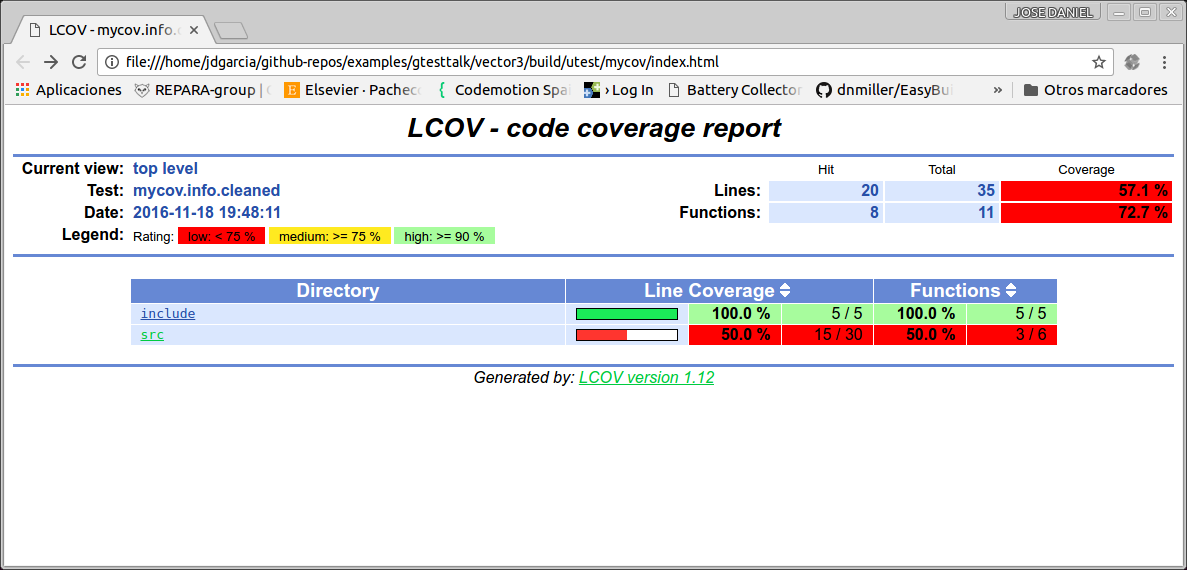
\includegraphics[width=\textwidth]{img/lcov1.png}
\end{frame}

\begin{frame}[t]{Generated report}
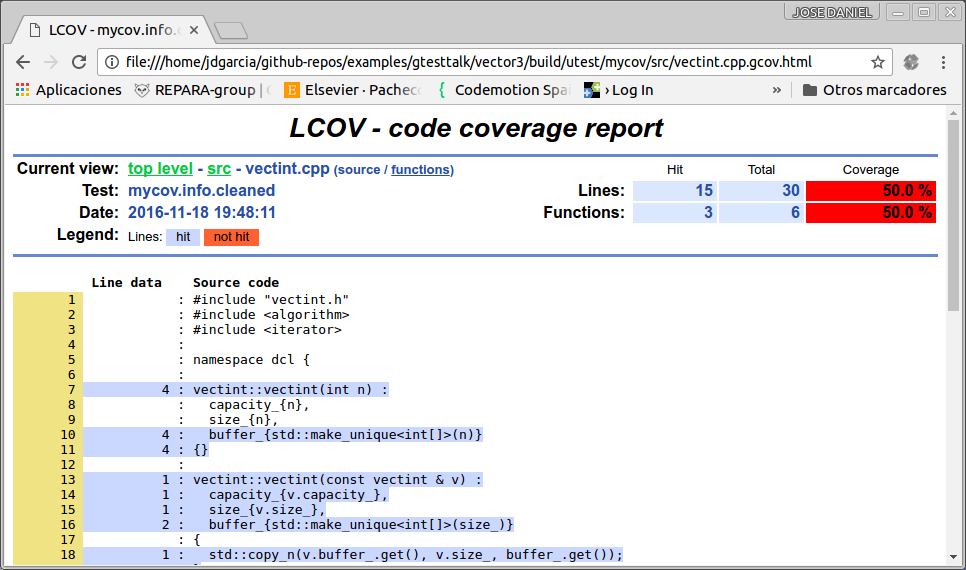
\includegraphics[width=\textwidth]{img/lcov2.png}
\end{frame}

\begin{frame}[t]{Generated report}
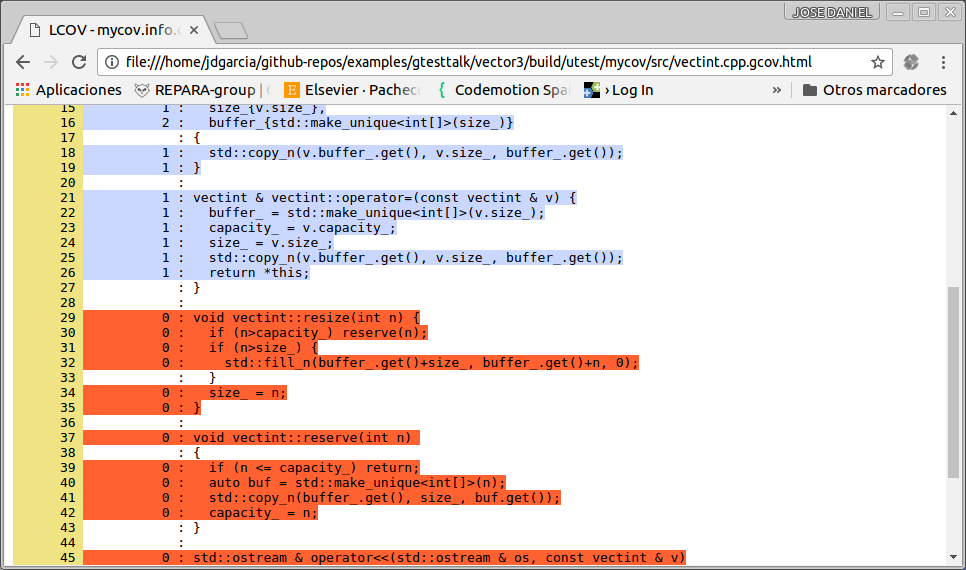
\includegraphics[width=\textwidth]{img/lcov3.png}
\end{frame}


\section{More unit tests}

\subsection{Test Fixtures}

\begin{frame}[t]{What is a Fixture?}
\begin{itemize}
  \item A test case with the same object configuration for all tests.
    \begin{itemize}
      \item Allows to avoid writing repetitive code to set up tests.
    \end{itemize}

  \item How?
    \begin{itemize}
      \item Define a class with the name of the case derived from
            \cppid{::testing::Test}.
      \item Make data members for objects that must be visible from tests.
      \item Define constructor and/or destructor.
        \begin{itemize}
          \item Alternatively \cppid{SetUp()} and/or \cppid{TearDown()}.
        \end{itemize}
      \item Use macro \cppid{TEST\_F} instead of \cppid{TEST}.
    \end{itemize}
\end{itemize}
\end{frame}

\begin{frame}[t]{My first Fixture}
\begin{block}{vectint\_copy}
\lstinputlisting[lastline=12]{examples/vector4/utest/vectint_copy.cpp}
\end{block}
\end{frame}

\begin{frame}[t]{My first Fixture}
\begin{columns}

\column{.5\textwidth}
\begin{block}{vectint\_copy}
\lstinputlisting[firstline=14,lastline=23]{examples/vector4/utest/vectint_copy.cpp}
\end{block}

\column{.5\textwidth}
\begin{block}{vectint\_copy}
\lstinputlisting[firstline=14,lastline=23]{examples/vector4/utest/vectint_copy.cpp}
\end{block}

\end{columns}
\end{frame}

\subsection{Completing tests}

\begin{frame}[t]{Testing size and capacity}
\begin{columns}[T]

\column{.6\textwidth}
\begin{block}{utest/vectint\_sizing.cpp}
\lstinputlisting[lastline=15]{examples/vector4/utest/vectint_sizing.cpp}
\end{block}

\column{.4\textwidth}
\begin{block}{utest/vectint\_sizing.cpp}
\lstinputlisting[firstline=17,lastline=25]{examples/vector4/utest/vectint_sizing.cpp}
\end{block}

\end{columns}
\end{frame}

\begin{frame}[t]{Testing capacity}
\begin{block}{utest/vectint\_sizing.cpp}
\lstinputlisting[firstline=27,lastline=41]{examples/vector4/utest/vectint_sizing.cpp}
\end{block}
\end{frame}

\begin{frame}[t]{Testing size}
\begin{block}{utest/vectint\_sizing.cpp}
\lstinputlisting[firstline=43,lastline=59]{examples/vector4/utest/vectint_sizing.cpp}
\end{block}
\end{frame}

\begin{frame}[t]{Testing size}
\begin{block}{utest/vectint\_sizing.cpp}
\lstinputlisting[firstline=61]{examples/vector4/utest/vectint_sizing.cpp}
\end{block}
\end{frame}

\begin{frame}[t]{Testing size}
\begin{block}{utest/vectint\_sizing.cpp}
\lstinputlisting[firstline=43,lastline=59]{examples/vector4/utest/vectint_sizing.cpp}
\end{block}
\end{frame}

\begin{frame}[t,fragile]{Running tests}
\begin{lstlisting}[style=terminal,basicstyle=\tiny\ttfamily]
jdgarcia@gavilan:~/vector4/build\$ ctest
Test project /home/jdgarcia/bitbucket-repos/charlas-es/codemotion-16-gtest/examples/vector4/build
    Start 1: vectint_sizing.reserve_grow
1/9 Test #1: vectint_sizing.reserve_grow .................   Passed    0.00 sec
    Start 2: vectint_sizing.reserve_shrink
2/9 Test #2: vectint_sizing.reserve_shrink ...............   Passed    0.00 sec
    Start 3: vectint_sizing.resize_grow_over_capacity
3/9 Test #3: vectint_sizing.resize_grow_over_capacity ....***Exception: SegFault  0.10 sec
    Start 4: vectint_sizing.resize_grow_under_capacity
4/9 Test #4: vectint_sizing.resize_grow_under_capacity ...***Exception: SegFault  0.10 sec
    Start 5: vectint_sizing.resize_shrink
5/9 Test #5: vectint_sizing.resize_shrink ................   Passed    0.00 sec
    Start 6: vectint_copy.copy_construct
6/9 Test #6: vectint_copy.copy_construct .................   Passed    0.00 sec
    Start 7: vectint_copy.copy_assign
7/9 Test #7: vectint_copy.copy_assign ....................   Passed    0.00 sec
    Start 8: vectint_constructor.empty
8/9 Test #8: vectint_constructor.empty ...................   Passed    0.00 sec
    Start 9: vectint_constructor.sized
9/9 Test #9: vectint_constructor.sized ...................   Passed    0.00 sec
\end{lstlisting}
\end{frame}

\begin{frame}[t,fragile]{Running tests}
\begin{lstlisting}[style=terminal,basicstyle=\tiny\ttfamily]
78% tests passed, 2 tests failed out of 9

Total Test time (real) =   0.21 sec

The following tests FAILED:
	  3 - vectint_sizing.resize_grow_over_capacity (SEGFAULT)
	  4 - vectint_sizing.resize_grow_under_capacity (SEGFAULT)
Errors while running CTest
\end{lstlisting}
\end{frame}

\begin{frame}[t,fragile]{Running a specific case}
\begin{itemize}
  \item A specific case can be selected.
    \begin{itemize}
      \item Option \cppkey{- -gtest\_filter="vectint\_sizing.*"}
    \end{itemize}
\end{itemize}
\begin{lstlisting}[style=terminal,basicstyle=\tiny\ttfamily]
jdgarcia@gavilan:~/vector4/build$ ./vectint_utest --gtest_filter="vectint_sizing.*"Running main() from gtest_main.cc
Note: Google Test filter = vectint_sizing.*
[==========] Running 5 tests from 1 test case.
[----------] Global test environment set-up.
[----------] 5 tests from vectint_sizing
[ RUN      ] vectint_sizing.reserve_grow
[       OK ] vectint_sizing.reserve_grow (0 ms)
[ RUN      ] vectint_sizing.reserve_shrink
[       OK ] vectint_sizing.reserve_shrink (0 ms)
[ RUN      ] vectint_sizing.resize_grow_over_capacity
Violación de segmento (`core' generado)
\end{lstlisting}
\end{frame}

\begin{frame}[t,fragile]{Running a specific test}
\begin{itemize}
  \item A specific test can be selected.
    \begin{itemize}
      \item Option \cppkey{- -gtest\_filter="vectint\_sizing.resize\_grow\_over\_capacity"}
    \end{itemize}
\end{itemize}
\begin{lstlisting}[style=terminal,basicstyle=\tiny\ttfamily]
jdgarcia@gavilan:~/vector4/build$ ./vectint_utest --gtest_filter="vectint_sizing.resize_grow_over_capacity"
Running main() from gtest_main.cc
Note: Google Test filter = vectint_sizing.resize_grow_over_capacity
[==========] Running 1 test from 1 test case.
[----------] Global test environment set-up.
[----------] 1 test from vectint_sizing
[ RUN      ] vectint_sizing.resize_grow_over_capacity
Violación de segmento (`core' generado)
\end{lstlisting}
\end{frame}

\begin{frame}[t]{Error in resize()}
\begin{block}{resize()}
\lstinputlisting[firstline=29,lastline=35]{examples/vector4/src/vectint.cpp}
\end{block}
\end{frame}

\begin{frame}[t]{Fixing resize()}
\begin{block}{resize()}
\lstinputlisting[firstline=29,lastline=35]{examples/vector5/src/vectint.cpp}
\end{block}
\end{frame}

\begin{frame}[t]{Error in reserve()}
\begin{block}{reserve()}
\lstinputlisting[firstline=37,lastline=44]{examples/vector4/src/vectint.cpp}
\end{block}
\end{frame}

\begin{frame}[t]{Fixing reserve()}
\begin{block}{reserve()}
\lstinputlisting[firstline=37,lastline=44]{examples/vector5/src/vectint.cpp}
\end{block}
\end{frame}

\subsection{Testing input/output}

\begin{frame}[t]{Testing streams}
\begin{itemize}
  \item Streams are organized in a class hierarchy.
    \begin{itemize}
      \item \cppid{std::ostringstream} es a \cppid{std::ostream}.
    \end{itemize}
\end{itemize}
\vfill
\begin{block}{vectint\_io.cpp}
\lstinputlisting{examples/vector5/utest/vectint_io.cpp}
\end{block}
\end{frame}




\begin{frame}
\titlepage
\end{frame}

\end{document}
